%!TEX root = main.tex


\section{Probability with connectable submodels}

Throughout this paper, we will work with a restricted probability theory in which any measurable set $X$ to be a finite set. This is both because it makes explanations simpler and because it is easy to show that submodels exist in this setting (Lemma \ref{lem:subm_exist}). Many of the proofs in this paper (with the exception of the one just mentioned) can likely be specialised to more general probility theories due to our use of string diagrams developed for Markov categories.

The standard method of constructing probability models introduces a probability space $(\prob{P},(\Omega,\sigalg{F}))$ with $\Omega$ a sample space, $\sigalg{F}$ a $\sigma$-algebra on $\Omega$ and $\prob{P}$ a probability measure on $(\Omega,\sigalg{F})$. Random variables are defined by measurable functions on $\Omega$ and are given names in sans-serif like $\RV{X}$. A probability distribution $\prob{P}^{\RV{XYZ}}$ is ``the joint distribution of $\RV{X}$, $\RV{Y}$ and $\RV{Z}$ under $\prob{P}$'' where $\RV{X},$ $\RV{Y}$ and $\RV{Z}$ are associated with random variables on $\Omega$ and is given by the pushforward of the function $\omega\mapsto (\RV{X}(\omega),\RV{Y}(\omega),\RV{Z}(\omega))$. Unless otherwise stated, a random variable named $\RV{X}$ will take values in the space $X$ (note the serif font).

To help us to construct causal models, we need an alternative method for building probability models. The motivation for doing this is to make it easy to represent a certain type of operation common in causal models. It is well-known that causal models make use of operations that are not standard in probability theory. For example, in the causal graphical model framework, given $\prob{P}^{\RV{XYZ}}$, if $\RV{Z}$ blocks a backdoor path between $\RV{X}$ and $\RV{Y}$ then the backdoor adjustment formula allows us to define a new probability space with measure $\prob{P}_x$ via ``truncated factorisation'' \citep[page ~24]{pearl_causality:_2009}:

\begin{align}
	\prob{P}^{\RV{YZ}}_{x}(y,z):=\prob{P}^{\RV{Y|XZ}}(y|x,z)\prob{P}^{\RV{Z}}(z)\label{eq:truncated_fac}
\end{align}

The standard theory of probability does not assign any special siginificance to the expression on the right side of Equation \ref{eq:truncated_fac}. At the same time, the notation we have chosen for the left side of Equation \ref{eq:truncated_fac} implicitly claims that $\prob{P}^{\RV{YZ}}_{x}$ is a distribution over the same variables $\RV{Y}$ and $\RV{Z}$ as the original $\prob{P}^{\RV{XYZ}}$. One way we can make sense of this is if $\prob{P}_{x}$ is defined on the same sample space as the original $\prob{P}$, and $\RV{Y}$ and $\RV{Z}$ are the same measurable functions on $\Omega$. However, we need to be careful that Equation \ref{eq:truncated_fac} is not therefore a contradiction. For example, if $\RV{X}=\RV{Z}$ (as in, $\RV{X}$ and $\RV{Z}$ are \emph{the same function on }$\Omega$) then there will generally be no measure $\prob{P}_x$ such that $\prob{P}^{\RV{YZ}}_{x}(y,z)$ agrees with Equation \ref{eq:truncated_fac}.

We want to be able to define operations like Equation \ref{eq:truncated_fac}, and we want to keep the idea that the measure that results from this operation is a joint distribution over the ``same variables''. We do this by distinguishing \emph{variable names} from the functions used to represent the variables on a particular sample space. In our framework, variables are measurable functions \emph{with names}; most measurable functions will not be given a name, and so are not variables. We note that this is implicitly accomplished by the Structural Causal Model framework, in which ``intervention'' takes a variable named $\RV{X}$ associated with a function $f:\Omega\to X$ and replaces this with a different function $g:\Omega \to X$ associated with the same variable $\RV{X}$. This operation cannot be defined with an ``anonymous function'' because there is no name enabling a statement like ``this new function $g$ points to the same thing the old function $f$ did''. Consequently, ``variable names'' are an integral part of Structural Causal Models.

\subsection{Markov categories}
The basic elements we will work with are finite sets and Markov kernels. A Markov kernel $\kernel{K}:X\to \Delta(Y)$ is a map from $X$ to probability distributions on $Y$. We can represent it concretely by the elements $(\kernel{K}_{x}^y)_{x\in X, y\in Y}$. An element $K_x^y$ represents the probability of $y\in Y$ given the argument $x\in X$. In general, an argument $w$ appearing as a superscript can be read as ``the probability of $w$'' and an argument $v$ appearing as a subscript can be read as ``given $v$''. Note that we do \emph{not} use Einstein summation in any expressions in this paper -- all sums will be written out explicitly.

A Markov kernel must have the following properties:
\begin{align}
	0\leq &K_{x}^y \leq 1 &\forall x,y\\
	\sum_{y\in Y} K_{x}^y &= 1 & \forall x
\end{align}

A probability distribution is a Markov kernel $\kernel{P}:\{*\}\to \Delta(Y)$ where $\{*\}$ is a one-element set. Such a Markov kernel can be represented as a matrix with one row, i.e. a column vector.

We define two particular Markov kernels that play a special role. The erase map $\stopper{0.3}:X\to \{*\}$ is represented by the matrix $\stopper{0.3}_x = 1$ for all $x\in X$. It maps every element of $X$ to the unique probability distribution on $\{*\}$, which gives probability 1 to $*$, the only element of the set; we can think of this as forgetting the input.

The copy map $\splitter{0.15}: X\to \Delta(X\times X)$ is the Markov kernel represented by the matrix $\splitter{0.15}_x^{x',x''}:= \llbracket x = x' \rrbracket \llbracket x=x''\rrbracket$, where the iverson bracket $\llbracket \cdot \rrbracket$ evaluates to $1$ if $\cdot$ is true and $0$ otherwise. We can think of the copy map as taking an element $x$ and outputting a joint distribution of two ``variables'' that are deterministically equal to $x$.

A swap map $\swap{0.2}: X\times Y \to \Delta(Y\times X)$ is the Markov kernel represented by the matrix $\swap{0.2}_{x,y}^{y',x'}:=\llbracket x=x' \rrbracket \llbracket y=y'\rrbracket$. It takes two inputs and returns a joint distribution on two ``variables'' deterministically equal to the swapped inputs.

The category with finite sets as objects, Markov kernels as morphisms, matrix products as the composition operation, $\stopper{0.3}$ as the counit and $\splitter{0.15}$ as the comultiplication forms the category FinStoch. This is not a category theory paper, but the fact that we are working in this category has a practical consequence. FinStoch is a \emph{Markov category}, as defined by \citet{fritz_synthetic_2020} and discussed earlier by \citet{cho_disintegration_2019,fong_causal_2013}. All Markov categories share a formal system of ``string diagrams'' such that a valid derivation using the diagrammatic notation corresponds to a valid theorem in the category. Markov categories include categories more general than ours, such as the category with general measurable sets as objects and Markov kernels as morphisms.

\subsection{Graphical notation for Markov categories}

\todo[inline]{In an appendix, state the axioms of Markov categories and maybe a short tutorial on reading diagrams}

We represent a Markov kernel as a box and a probability distribution as a triangle:

\begin{align}
\kernel{K}&:=\begin{tikzpicture}[baseline={([yshift=-.5ex]current bounding box.center)}]
	\path (0,0) node (A) {}
	++ (0.5,0) node[kernel] (K) {$\kernel{K}$}
	++ (0.5,0) node (B) {};
	\draw (A) -- (K) -- (B);
\end{tikzpicture}\\
\prob{P}&:= \begin{tikzpicture}[baseline={([yshift=-.5ex]current bounding box.center)}]
	\path (0,0) node[dist] (K) {$\kernel{K}$}
	++ (0.5,0) node (B) {};
	\draw (K) -- (B);
\end{tikzpicture}
\end{align}

Two Markov kernels $\kernel{L}:X\to \Delta(Y)$ and $\kernel{M}:Y\to \Delta(Z)$ have a product $\kernel{L}\kernel{M}:X\to \Delta(Z)$ given by the matrix product: $\kernel{L}\kernel{M}_x^z = \sum_y \kernel{L}_x^y\kernel{M}_y^z$. Graphically, we write represent products by joining kernel wires together:

\begin{align}
	\kernel{L}\kernel{M}:= \begin{tikzpicture}[baseline={([yshift=-.5ex]current bounding box.center)}]
	\path (0,0) node (A) {}
	++ (0.5,0) node[kernel] (K) {$\kernel{K}$}
	++ (0.7,0) node[kernel] (M) {$\kernel{M}$}
	++ (0.5,0) node (B) {};
	\draw (A) -- (K) -- (M) -- (B);
\end{tikzpicture}
\end{align}

We read diagrams from left to right (this is somewhat different to \citet{fritz_synthetic_2020,cho_disintegration_2019,fong_causal_2013} but in line with \citet{selinger_survey_2010}). They are to be read as a series of products of Markov kernels. For some special Markov kernels, we can replace the generic ``box'' of a Markov kernel with a special diagrammatic element that is visually suggestive of what they accomplish.

The Cartesian product $X\times Y:=\{(x,y)|x\in X, y\in Y\}$.

Given kernels $\kernel{K}:W\to Y$ and $\kernel{L}:X\to Z$, the tensor product $\kernel{K}\otimes\kernel{L}:W\times X\to \Delta(Y\times Z)$ is defined by $(\kernel{K}\otimes\kernel{L})_{(w,x)}^{(y,z)}:=K_{w}^y L_{x}^z$.

The tensor product is represeted by parallel juxtaposition:

\begin{align}
	\kernel{K}\otimes \kernel{L}&:=\begin{tikzpicture}[baseline={([yshift=-.5ex]current bounding box.center)}]
	\path (0,0) node (A) {}
	++ (0.5,0) node[kernel] (K) {$\kernel{K}$}
	++ (0.5,0) node (B) {};
	\path (0,-0.5) node (C) {}
	++ (0.5,0) node[kernel] (L) {$\kernel{L}$}
	++ (0.5,0) node (D) {};
	\draw (A) -- (K) -- (B);
	\draw (C) -- (L) -- (D);
\end{tikzpicture}
\end{align}

The identity map is a bare line:

\begin{align}
	\mathrm{Id}&:=\begin{tikzpicture}[baseline={([yshift=-.5ex]current bounding box.center)}]
	\path (0,0) ++ (0.5,0) node (B) {};
	\draw (A) -- (B);
\end{tikzpicture}
\end{align}

The stopper is a fuse:

\begin{align}
	\stopper{0.3}&:=\begin{tikzpicture}[baseline={([yshift=-.5ex]current bounding box.center)}]
	\path (0,0) ++ (1,0) node (B) {};
	\draw[-{Rays[n=8]}] (A) -- (B);
\end{tikzpicture}
\end{align}

The splitter is a fork:

\begin{align}
	\splitter{0.2}&:=\begin{tikzpicture}[baseline={([yshift=-.5ex]current bounding box.center)}]
	\path (0,0) node (A) {} 
	++ (0.5,0) node[copymap] (copy0) {}
	++ (0.5,0.15) node (B) {}
	+ (0,-0.3) node (C) {};
	\draw (A) -- (copy0) to [out=45,in=180] (B) (copy0) to [out=-45, in=180] (C);
\end{tikzpicture}
\end{align}

The swap map swaps wires:

\begin{align}
	\swap{0.2} &:=  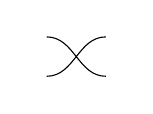
\begin{tikzpicture}[baseline={([yshift=-.5ex]current bounding box.center)}]
		\path (0,0) node (A) {} 
		+ (0,-0.5) node (B) {}
		++ (1,0) node (C) {}
		+ (0,-0.5) node (D) {};
		\draw (A) to [out=0,in=180] (D) (B) to [out=0, in=180] (C);
	\end{tikzpicture}
\end{align}

We will use the graphical notation for derivations, but because it is quite unfamiliar we will also include translations to more familiar notation.

\subsection{Revisiting truncated factorisation}

Recall the original problem of defining operations like Equation \ref{eq:truncated_fac}. We can seemingly do this quite easily using the tools of the FinStoch category. Note that $P^{\RV{Y|XZ}}$ must be represented by a Markov kernel $\kernel{K}:X\times Z\to \Delta(Y)$ and $\prob{P}^{\RV{Z}}$ by a Markov kernel $\kernel{L}\in \Delta(Z)$ (we will explain later why we explicitly distinguish Markov kernels from conditional probabilities). Then it seems that we can define a Markov kernel $\kernel{M}:X\to \Delta(X\times Z)$ representing $x\mapsto \prob{P}^{\RV{YZ}}_{x}(y,z)$ by

\begin{align}
	\kernel{M}:= \tikzfig{truncated_factorisation}\label{eq:tfac_setted}
\end{align}

There is a problem, however: in the diagram above $X$, $Y$ and $Z$ refer to the \emph{sets in which variables take values}, which are not an adequate substitute for variable labels. For example, if $\RV{X}_1$ and $\RV{X}_2$ both take values in $X$, then a Markov kernel $\kernel{K}$ representing some $\prob{P}^{\RV{X_1X_2}}$ could be drawn

\begin{align}
	\kernel{K}:= \tikzfig{double_label}
\end{align}

However the variable associated with each wire is different. Our solution to this is to give labels to sets. A labeled set is a set together with a label, such as $(\RV{X}_1,X)$, which can be read as the set of statements ``$\RV{X}_1=x$'' for each $x\in X$. In fact, we allow sets to have multiple synonymous labels $(\{\RV{X}_1,\RV{Q}\},X)$, which can be read as stipulating that $\RV{X}_1$ and $\RV{Q}$ refer to the same thing. In general, any two labels that appear in the same label set are called \emph{synonyms}.

Let $N_{\RV{X}}$ refer to the set of labels of $\RV{X}$. Any collection of labeled sets must live in a ``labelspace'' that prevents us from making inadmissible label assignments. We require the following axioms to hold for labeled sets occupying the same labelspace:

\begin{enumerate}
	\item \textbf{Uniqueness of labels:} Given two labeled sets $(N_1,X)$ and $(N_2,Y)$, if there exists some $\RV{W}\in N_1$ and $\RV{W}\in N_2$ then $N_1=N_2$ and $X=Y$
	\item \textbf{Empty label:} There is a unique empty label $*$ which is always associated with a 1-element set $\{*\}$
\end{enumerate}

Due to Axiom 1, we can unambiguously refer to a labeled set $(N_1,X)$ by any of its labels $\RV{X}\in N_1$. 

We define a \emph{sequence} of labeled sets

\begin{itemize}
	\item \textbf{Sequence of labeled sets:} Given $(N_\RV{X},X)$ and $(N_{\RV{Y}},Y)$ with $\RV{X}\in N_\RV{X}$ and $\RV{Y}\in N_{\RV{Y}}$, the sequence $(\RV{X}, \RV{Y})$ is the labeled set $(N,X\times Y)$ with $(\RV{X},\RV{Y})\in N$
\end{itemize}

Note that $(\RV{X},\RV{Y})$ is also a label. $(\RV{X},\RV{Y})$ may have synonyms such as $\RV{Z}$. We say a label $\RV{U}$ is \emph{atomic} if none of its synonyms are sequences of labels.

For some $\RV{W}$, we use $m_{\RV{W}}(\RV{Z})$ to refer to ``the number of times $\RV{W}$ appears in $\RV{Z}$''. We define this as follows:

\begin{itemize}
	\item $m_{\RV{W}}(\RV{Z})=1$ if $\RV{W}$ is a synonym of $\RV{Z}$
	\item $m_\RV{W}(\RV{Z})=0$ if $\RV{Z}$ is atomic and $\RV{W}$ is not a synonym of $\RV{Z}$
	\item Otherwise, if $\RV{Z}$ is synonymous with $(\RV{X},\RV{Y})$ then $m_{\RV{W}}(\RV{Z})=\argmax_{\RV{X}'\in N_{\RV{X}}} m_{\RV{W}}(\RV{X}') + \argmax_{\RV{Y}'\in N_{\RV{Y}}} m_{\RV{W}}(\RV{Y}')$
\end{itemize}

\todo[inline]{It's not obvious that this is unique}

We say $\RV{X}$ is in $\RV{Y}$ or $\RV{X}\in \RV{Y}$ if $m_{\RV{X}}(\RV{Y})>0$. We say that $*$ is in every sequence.

With this in mind, we define the following operations on sequences of labels

\begin{enumerate}
	\item \textbf{Difference of labels:} Given $\RV{X}$, $\RV{Y}$, the difference $\RV{X}\setminus \RV{Y}$ is a label sequence $\RV{Z}$ such that for any label $\RV{X}_i$, $m_{\RV{X}_i}(\RV{Z}) = \max(0,m_{\RV{X}_i}(\RV{X})-m_{\RV{X}_i}(\RV{Y}))$
	\item \textbf{Intersection of labels:} Given $\RV{X}$, $\RV{Y}$, the intersection $\RV{X}\cap \RV{Y}$ is a label sequence $\RV{Z}$ such that for any label $\RV{X}_i$, $m_{\RV{X}_i}(\RV{Z}) = \min(m_{\RV{X}_i}(\RV{X}),m_{\RV{X}_i}(\RV{Y}))$
\end{enumerate}

These definitions are non-unique in that they do not define the order of $\RV{Z}$. This doesn't cause a problem because we work with labeled Markov kernels that we define to be equivalent if one can be obtained from the other by permuting its labels and applying the corresponding swap maps. We use the convention that $*$ is synonymous with a sequence under which every label has multiplicity 0.

\subsection{Labeled Markov kernels}\label{sec:labeled_kernels}

\todo[inline]{LabeledFinStoch is actually a different category to FinStoch and I have to show it satisfies the axioms of a Markov category}

A labeled Markov kernel $\kernel{K}:\RV{A}\to \Delta(\RV{B})$ is a Markov kernel that maps between labeled sets. If $\RV{A}$ takes values in $X$ and $\RV{B}$ takes values in $Y$, then $\kernel{K}$ is the underlying Markov kernel $\kernel{K'}:X\to \Delta(Y)$ along with the \emph{domain label} $\RV{A}$ and \emph{codomain label} $\RV{B}$. The labels $\RV{A}$ and $\RV{B}$ can be replaced by any synonyms of $\RV{A}$ and $\RV{B}$.

A labeled probability distribution $\prob{P}\in\Delta(Y)$ comes with a codomain label $(\RV{B})$ only.

Graphically, we annotate the wires of a labeled kernel with the corresponding labels. If $\kernel{K}:(\RV{A}_1,\RV{A}_2)\to \Delta(\RV{B}_1,\RV{B}_2)$, it is represented:

\begin{align}
	\kernel{K} := \begin{tikzpicture}[baseline={([yshift=-.5ex]current bounding box.center)}]
	\path (0,0) node (A1) {$\RV{A}_1$}
	+ (0,-0.3) node (A2) {$\RV{A}_2$}
	++ (0.7,-0.15) node[kernel] (K) {$\kernel{K}$}
	++ (0.7,0.15) node (B1) {$\RV{B}_1$}
	+ (0,-0.3) node (B2) {$\RV{B}_2$};
	\draw (A1) -- ($(K.west) + (0,0.15)$) (A2) -- ($(K.west) + (0,-0.15)$);
	\draw (B1) -- ($(K.east) + (0,0.15)$) (B2) -- ($(K.east) + (0,-0.15)$);
\end{tikzpicture}
\end{align}

We can also use single wires to represent sequences of labeled sets:

\begin{align}
	\kernel{K} = \begin{tikzpicture}[baseline={([yshift=-.5ex]current bounding box.center)}]
	\path (0,0) node (A1) {$(\RV{A}_1,\RV{A}_2)$}
	++ (1.3,0) node[kernel] (K) {$\kernel{K}[\model{L}]$}
	++ (1.3,0.) node (B1) {$(\RV{B}_1,\RV{B}_2)$};
	\draw (A1) -- (K) -- (B1);
\end{tikzpicture}
\end{align}

We say two labeled kernels $\kernel{K}$ and $\kernel{L}$ are equivalent if one can be obtained from the other by a permutation of labels and application of the corresponding swap maps. For example, if we have $\kernel{K}:(\RV{X},\RV{Y})\to \Delta(\RV{Z},\RV{W})$ and $\kernel{L}:(\RV{Y},\RV{X})\to \Delta(\RV{W},\RV{Z})$, then $\kernel{K}$ and $\kernel{L}$ are equivalent, written $\kernel{K}\overset{perm}{=}\kernel{L}$ if

\begin{align}
\tikzfig{equivalence}
\end{align}

A labeled Markov kernel must satisfy the following axiom. This axiom is what makes the use of labeled Markov kernels and labeled sets different to the use of ordinary Markov kernels and sets.

\begin{enumerate}
	\item For any labeled kernel $\kernel{K}:\RV{A}\to \Delta(\RV{B})$, there must be a valid diagrammatic representation in which all instances of the same label are connected by a path consisting of wires and copy maps only.
\end{enumerate}

For example, given $\kernel{K}:(\RV{X},\RV{Y})\to \Delta(\RV{X},\RV{Z})$, we require that there exist some $\kernel{H}:X\times Z\to \Delta(Y)$ such that
\begin{align}
	\kernel{K} &= \begin{tikzpicture}[baseline={([yshift=-.5ex]current bounding box.center)}]
					\path (0,0) node (X) {$\RV{X}$}
					+ (0,-0.65) node (Z) {$\RV{Z}$}
					++ (0.5,0) node[copymap] (copy0) {}
					++ (0.7,-0.5) node[kernel] (L) {$\kernel{H}$}
					++ (0.9,0.65) node (Xout) {$\RV{X}$}
					+  (0,-0.65) node (Y) {$\RV{Y}$};
					\draw (X) -- (copy0) to [out=-45,in=180] ($(L.west) + (0,0.15)$) (L) -- (Y);
					\draw (copy0) to [out=45,in=180] (Xout);
					\draw (Z) -- ($(L.west) + (0,-0.15)$);
				 \end{tikzpicture}\label{eq:extn1}\\
	 	&\iff\\
	 \kernel{K}_{xz}^{x'y} &= \llbracket x=x'\rrbracket \kernel{H}_{xz}^{y}
\end{align}

Note the path connecting the two instances of $\RV{X}$ goes only through a copy map. For a second example, given $\kernel{L}: \RV{Z}\to \Delta(\RV{X},\RV{X},\RV{Y})$, we require that there exist some $\kernel{G}:\RV{Z}\to \Delta(\RV{X}, \RV{Y})$ such that
\begin{align}
	\kernel{L} &= \begin{tikzpicture}[baseline={([yshift=-.5ex]current bounding box.center)}]
					\path (0,0) node (Z) {$\RV{Z}$}
					++ (0.9,0) node[kernel] (L) {$\kernel{G}$}
					++ (0.9,0.15) node[copymap] (copy0) {}
					++ (0.5,0.3) node (X1) {$\RV{X}$}
					++ (0,-0.3) node (X2) {$\RV{X}$}
					++  (0,-0.3) node (Y) {$\RV{Y}$};
					\draw ($(L.east) + (0,0.15)$) -- (copy0) to[out=0,in=180] (X2);
					\draw (copy0) to [out=45,in=180] (X1);
					\draw (Z)--(L) ($(L.east) + (0,-0.15)$) -- (Y);
				 \end{tikzpicture}\label{eq:extn2}\\
			   &\iff\\
		\kernel{L}_{z}^{xx'y} &= \llbracket x=x' \rrbracket\kernel{G}_{z}^{xy}	   
\end{align}

In short, \emph{instances of the same label must be deterministically equal}. Note that this axiom rules out the existence of any labeled kernels with multiple copies of the same label as inputs.

The \emph{connection} operation, defined in the next section, can compactly represent both cases above. If $\RV{X}$ is some label that appears twice in the output of $\kernel{L}$ or once in the input and once in the output, then there must be some $\kernel{M}$ such that

\begin{align}
	\kernel{L}=\kernel{M}\rightrightarrows\kernel{I}\label{eq:extn3}
\end{align}

\todo[inline]{I need to make this an axiom}

\subsection{Connection}

Connection is an associative operation $\rightrightarrows$ that ``joins'' two labeled Markov kernels where the labels can be matched and preserves unmatched inputs and outputs. A key property of connection is that, if both input Markov kernels satisfy Axiom 1, then the output also satisfies axiom 1. One can think of this operation like connecting two lego bricks of different sizes -- we connect all the parts that will fit together, and all the connection points that don't fit are left available.

Given two labeled Markov kernels $\kernel{F}:\RV{I}_F\to\Delta(\RV{O}_F)$ and $\kernel{S}:\RV{I}_S\to\Delta(\RV{O}_S)$, make the following label identifications:
\begin{align}
	\RV{O}_{F\cdot}&:=\RV{O}_F\setminus\RV{I}_S &\text{Labels only in the output of } \kernel{F}\\
	\RV{O}_{FS}&:=\RV{O}_F\cap\RV{I}_S &\text{Labels in the output of both}\\
	\RV{I}_{F\cdot} &:= \RV{I}_F\setminus \RV{I}_S &\text{Labels only in the input } \kernel{F}\\
	\RV{I}_{FS}&:= \RV{I}_F\cap\RV{I}_S &\text{Labels in the input of both}\\
	\RV{I}_{\cdot S}&:= \RV{I}_S\setminus \RV{I}_F &\text{Labels only in the input of }\kernel{S} \\
	\RV{O}_{I_FO_S*}&:=\RV{O}_S\cap \RV{I}_F\setminus \RV{I}_S &\text{Input of }\kernel{F}\text{ and the output only of }\kernel{S}\\
	\RV{O}_{O_FO_S*} &:= \RV{O}_F\cap\RV{O}_S\setminus \RV{I}_S&\text{Output of }\kernel{F}\text{ and the output only of }\kernel{S}\\
\end{align}

$\kernel{F}$ can be connected to $\kernel{S}$ iff $\RV{O}_{I_FO_S*}$ synonymous with $*$ and $\RV{O}_{O_FO_S*}$ is also synonymous with $*$. The reason for this is that, in general, if these sets were non-empty then we would not have a way to connect $\kernel{F}$ and $\kernel{S}$ without violating axiom 1.

\begin{definition}[connection]\label{def:extension}
Consider a labeled Markov kernel $\kernel{F}:\RV{I}_F\to\Delta(\RV{O}_F)$ which can be connected to $\kernel{S}:\RV{I}_S\to\Delta(\RV{O}_S)$. Because they can be conected, we can write $\kernel{F}:(\RV{I}_{F\cdot},\RV{I}_{FS})\to\Delta(\RV{O}_{F\cdot},\RV{O}_{FS}))$ and $\kernel{S}:(\RV{I}_{FS},\RV{I}_{\cdot S})\to\Delta(\RV{O}_S)$.

Then Equations \ref{eq:extn_definition1} and \ref{eq:extn_definition2} are equivalent definitions of extension:
\begin{align}
	\kernel{K}\rightrightarrows \kernel{L} &:=  \begin{tikzpicture}[baseline={([yshift=-.2ex]current bounding box.center)}]
		\path (0,0) node (Y) {$\RV{I}_{F\cdot}$}
		+ (0,-0.3) node (Q) {$\RV{I}_{FS}$}
		+ (0,-0.8) node (R) {$\RV{I}_{\cdot S}$}
		++ (0.5,-0.3) node[copymap] (copy0) {}
		++ (0.5,0.15) node[kernel] (K) {$\kernel{F}$}
		++ (0.5,-0.15) node[copymap] (copy1) {}
		++ (0.6,-0.5) node[kernel] (L) {$\kernel{S}$}
		++ (0.6, 0.8) node (Z) {$\RV{O}_{F\cdot}$}
		+ (0,-0.3) node (X) {$\RV{O}_{FS}$}
		+ (0,-0.8) node (W) {$\RV{O}_S$};
		\draw (Y) -- ($(K.west) + (0,0.15)$) (Q) -- ($(K.west) + (0,-0.15)$);
		\draw (copy0) to [out=-45,in=180] ($(L.west) + (0,0)$) (copy1) to [out=-60,in=180] ($(L.west) + (0,0.15)$);
		\draw (R) to [out=0,in=180] ($(L.west) + (0,-0.15)$);
		\draw ($(K.east) + (0,-0.15)$) to (copy1);
		\draw ($(K.east) + (0,0.15)$) -- (Z) (copy1) to [out=0,in=180] (X) (L) -- (W);
	\end{tikzpicture}\label{eq:extn_definition1}\\
	&:= \kernel{J}\\
	\kernel{J}_{yqr}^{zxw} &= \kernel{F}_{yq}^{zx} \kernel{S}_{xqr}^{w}\label{eq:extn_definition2}
\end{align}
Note that there are no sums in Equation \ref{eq:extn_definition1}, this is simply a product of matrix elements.
\end{definition}

\begin{lemma}[Connection is associative up to permuation of labels]\label{lem:con_associative}
Given labeled Markov kernels $\kernel{K}:\RV{I}_K\to\Delta(\RV{O}_K)$, $\kernel{L}:\RV{I}_L\to\Delta\RV{O}_L)$ and $\kernel{J}:\RV{I}_J\to\Delta(\RV{O}_J)$,
\begin{align}
	(\kernel{K}\rightrightarrows \kernel{L})\rightrightarrows \kernel{J} &\overset{perm}{=} \kernel{K}\rightrightarrows (\kernel{L}\rightrightarrows \kernel{J})
\end{align}
\end{lemma}

\begin{proof}
Proven in Appendix \ref{sec:connect_associative}
\end{proof}

\begin{lemma}[Identity maps commute one way with connection]
Consider the identity map on some labeled set $\kernel{I}:\RV{X}\to \Delta(\RV{X})$ (note that by Equation \ref{eq:extn1} the identity map is the \emph{only} kernel with this signature). For any $\kernel{M}:\RV{Y}\to\Delta(\RV{Z})$, either a copy of $\RV{X}$ appears in the output but not the input and $\kernel{I}\rightrightarrows \kernel{M}$ is undefined, or $\kernel{I}\rightrightarrows\kernel{M}=\kernel{M}\rightrightarrows\kernel{I}$.
\end{lemma}

\begin{proof}
Consider the identity map on some labeled set $\kernel{I}:\RV{X}\to \Delta(\RV{X})$ (note that by Equation \ref{eq:extn1} the identity map is the \emph{only} kernel with this signature). Note that for any $\kernel{M}:\RV{Y}\to\Delta(\RV{Z})$, either a copy of $\RV{X}$ appears in the output but not the input, in which case $\kernel{I}\rightrightarrows \kernel{M}$ is undefined, or we have one of the following cases:

If $\RV{X}$ is in $\RV{Y}$ and $\RV{Z}$, then there must be some $\kernel{N}$ such that Equation \ref{eq:extn1} holds. Defining $\RV{Y}'=\RV{Y}\setminus\RV{X}$ and $\RV{Z}'=\RV{Z}\setminus\RV{X}$:

\begin{align}
	\kernel{I}\rightrightarrows\kernel{M}&=\tikzfig{iconnectm}\\
										 &=\tikzfig{iconnectm_rev}\\
										 &=\kernel{M}\rightrightarrows\kernel{I}
\end{align}

\todo[inline]{Commutativity of copy map in appendix}

If $\RV{X}$ is in $\RV{Y}$ only, defining $\RV{Y}'=\RV{Y}\setminus\RV{X}$:

\begin{align}
	\kernel{I}\rightrightarrows\kernel{M}&=\tikzfig{iconnectm_clear}\\
										 &=\kernel{M}\rightrightarrows\kernel{I}
\end{align}

If $\RV{X}$ is in neither $\RV{Y}$ nor $\RV{Z}$, then

\begin{align}
	\kernel{I}\rightrightarrows\kernel{M}&=\tikzfig{iconnectm_dclear}\\
										 &=\kernel{M}\rightrightarrows\kernel{I}
\end{align}
\end{proof}

\begin{theorem}[Connection is compatible with axiom 1]
Given $\kernel{K}:\RV{A}\to\Delta(\RV{B})$ and $\kernel{L}:\RV{C}\to\Delta(\RV{D})$, let $\kernel{J}=\kernel{K}\rightrightarrows \kernel{L}$. Then $\kernel{J}$ satisfies axiom 1.
\end{theorem}

\begin{proof}
By inspecting the definition of $\rightrightarrows$ (Equation \ref{eq:extn_definition1}), we can see that no labels from either of the inputs are increased in multiplicity. We need to verify that if either of the inputs has a label with multiplicity $>1$, then the result of the extension still satisfies axiom 1. 

Consider any label $\RV{X}$ that appears in both the input and output of $\kernel{K}$, or twice in the output of $\kernel{K}$. Then Equation \ref{eq:extn3} implies that there exists some $\kernel{H}$ such that $\kernel{K}=\kernel{H}\rightrightarrows\kernel{I}$.

Thus

\begin{align}
	\kernel{K}\rightrightarrows \kernel{L} &= (\kernel{H}\rightrightarrows \kernel{I})\rightrightarrows\kernel{L}\\
										   &\overset{perm}{=} \kernel{H}\rightrightarrows(\kernel{I}\rightrightarrows\kernel{L})\\
										   &= \kernel{H}\rightrightarrows(\kernel{L}\rightrightarrows\kernel{I})\\
										   &\overset{perm}{=} (\kernel{H}\rightrightarrows\kernel{L})\rightrightarrows\kernel{I}
\end{align}

Which implies that $\kernel{J}$ satistfies Equation \ref{eq:extn3} for $\RV{Y}$.

Consider $\RV{Z}$ that appears in the input and output of $\kernel{L}$ or twice in the output of $\kernel{L}$. Then there exists some $\kernel{G}$ such that

\begin{align}
	\kernel{K}\rightrightarrows \kernel{L} &= \kernel{K}\rightrightarrows (\kernel{G}\rightrightarrows\kernel{I})\\
										   &\overset{perm}{=} (\kernel{K}\rightrightarrows \kernel{G})\rightrightarrows\kernel{I}
\end{align}

Which implies $\kernel{J}$ satisfies Equation \ref{eq:extn3}.
\end{proof}

\subsection{Submodels}

Note that at this point, we have a theory of probability that can handle Equation \ref{eq:truncated_fac}. In particular, $P^{\RV{Y|XZ}}$ must be represented by a labeled Markov kernel $\kernel{K}:(\RV{X}, \RV{Z})\to \Delta(\RV{Y})$ and $\prob{P}^{\RV{Z}}$ by a labeled Markov kernel $\kernel{L}\in \Delta(\RV{Z})$. Then we can define a labeled Markov kernel $\kernel{M}:\RV{X}\to \Delta(\RV{X}, \RV{Z})$ representing $x\mapsto \prob{P}^{\RV{YZ}}_{x}(y,z)$ by

\begin{align}
	\kernel{M}&:= \kernel{L}\rightrightarrows\kernel{K}\\
	 		&=\tikzfig{truncated_factorisation_labeled}\label{eq:tfac_labeled}
\end{align}

We can see that Equation \ref{eq:tfac_labeled} is almost identical to Equation \ref{eq:tfac_setted} except with set labels instead of sets annotating the wires. This minor change, along with Axiom 1, deals with the problem of identical sets previously mentioned.

However, we do not yet have a notion of \emph{marginal probability} or \emph{conditional probability}. In the paragraph above, the terms $P^{\RV{Y|XZ}}$ and $\prob{P}^{\RV{Z}}$ are external to the theory developed so far. However, we do know that they are related in a particular way; namely, they are respectively a contitional distribution and a marginal distribution derived from the same probability space with measure $P$. 

We will use the term \emph{submodels} to refer to marginals and conditionals of a higher level model, like those mentioned in the previous paragraph. 

\begin{definition}[Marginal]
For any label $\RV{X}$, define the marginalising kernel $\stopper{0.3}_{\RV{X}}:\RV{X}\to *$, which is necessarily unique. Given $\kernel{K}:\RV{W}\to\Delta(\RV{Y})$ and $\kernel{L}:\RV{W}\to \Delta(\RV{Z})$, $\RV{L}$ is a \emph{marginal} of $\kernel{K}$ if, for some $\RV{X}$ in $\RV{Y}$,
\begin{align}
	\kernel{K}\rightrightarrows\stopper{0.3}_{\RV{X}} = \kernel{L}
\end{align}
\end{definition}

Because $*$ is in every sequence of labels, $\kernel{K}$ is always a marginal of itself.

\begin{definition}[Submodel]
Given $\kernel{K}:\RV{X}\to \Delta(\RV{Y})$ and $\kernel{L}:\RV{W}\to\Delta(\RV{Z})$, $\kernel{L}$ is a submodel of $\kernel{K}$ if there are marginals $\kernel{K}'$, $\kernel{K}''$ of $\kernel{K}$ such that
\begin{align}
	 \kernel{K}'\rightrightarrows\kernel{L} = \kernel{K}''
\end{align}
\end{definition}

As the trivial map $\stopper{0.3}:\RV{X}\to\Delta(\{*\})$ is a marginal of $\kernel{K}$, and $\stopper{0.3}\rightrightarrows\kernel{K}'=\kernel{K}'$ for any marginal of $\kernel{K}$, every marginal of $\kernel{K}$ is also a submodel of $\kernel{K}$.

With the definition of submodels in hand, we can introduce a notation more familiar to people experienced with probability theory. If $\kernel{L}:\RV{X}\to \Delta(\RV{Y})$ is a submodel of $\kernel{K}$, we may write $\kernel{L}\equiv \model{K}^{\RV{Y}|\RV{X};\kernel{L}}$ and $\kernel{L}_x^y\equiv \model{K}^{\RV{Y}|\RV{X};\kernel{L}}(y|x)$. Note that the same kernel might be a submodel of many other kernels. This notation isn't \emph{entirely} familiar, as we retain a reference to the original kernel $\kernel{L}$. In general, a kernel $\kernel{K}$ has many submodels with the same signature, and this non-uniqueness is more problematic for causal models than for standard probabilistic models, as we will see in Section \ref{sec:CBN}.

\begin{lemma}[Submodel existence]\label{lem:subm_exist}
In FinStoch, for any $\kernel{K}:\RV{W}\to \Delta(\RV{X},\RV{Y})$ there exists a submodel $\model{K}^{\RV{Y}|\RV{XW};\kernel{L}}$.
\end{lemma}

\begin{proof}
Consider any Markov kernel $\kernel{L}:(\RV{X},\RV{W})\to \Delta(\RV{Y})$ with the property
\begin{align}
	\kernel{L}_{xw}^{y} = \frac{\kernel{K}_w^{xy}}{\sum_{x\in X}\kernel{K}_w^{xy}}\qquad\forall {w,y}:\text{ the denominator is positive}
\end{align}

Then define $\kernel{K}^{\RV{X}|\RV{W};\kernel{M}}:=\kernel{K}\rightrightarrows\stopper{0.3}_{\RV{Y}}$, which is a marginal of $\kernel{K}$. THen
\begin{align}
	(\kernel{M}\rightrightarrows\kernel{L})_w^{xy} &= \kernel{M}_w^x\kernel{L}_{xw}^y&\\
												   &= \sum_{x\in X} \kernel{K}_w^{xy} \frac{\kernel{K}_w^{xy}}{\sum_{x\in X}\kernel{K}_w^{xy}} &\text{ if }\kernel{K}_w^{xy}>0\\
												   &= \kernel{K}_w^{xy} &\text{ if }\kernel{K}_w^{xy}>0\\
												   &= 0 &\text{otherwise}\\
												   &= \kernel{K}_w^{xy} &\text{otherwise}
\end{align}
\end{proof}

We did not use string diagrams in this proof, so this result does not necessarily apply to other Markov kernel categories. This is the technical reason why we choose to work with FinStoch: the existence of submodels presents a challenge in more general settings that we haven't fully resolved and the progress we have is beyond the scope of this paper.

\subsection{Conditional independence}\label{ssec:cond_indep}

We define conditional independence in the following manner:

For a \emph{probability distribution} $\kernel{P}:\{*\}\to \Delta(\RV{Y})$ and some $\RV{A},\RV{B},\RV{C}\in \RV{Y}$, we say $\RV{A}$ is independent of $\RV{B}$ given $\RV{C}$, written $\RV{A}\CI_{\kernel{P}}\RV{B}|\RV{C}$, if there are submodels $\model{P}^{\RV{ABC};\kernel{J}}$, $\model{P}^{\RV{C};\kernel{K}}$, $\model{P}^{\RV{A}|\RV{C};\kernel{L}}$, $\model{P}^{\RV{B}|\RV{C};\kernel{M}}$ such that

\begin{align}
	\kernel{P}^{\RV{ABC};\kernel{J}} &= \tikzfig{cond_indep1}
\end{align}

For a \emph{kernel} $\kernel{N}:\RV{X}\to \Delta(\RV{Y})$ and some $\RV{A},\RV{B},\RV{C}\in (\RV{X},\RV{Y})$, we say $\RV{A}$ is independent of $\RV{B}$ given $\RV{C}$, written $\RV{A}\CI_{\kernel{N}}\RV{B}|\RV{C}$, if there is some $\kernel{O}:\{*\}\to \Delta(\RV{X})$ such that $O^x>0$ for all $x\in X$ and $\RV{A}\CI_{\kernel{O}\rightrightarrows\kernel{N}} \RV{B}|\RV{C}$.

This definition is inappliccable in the case where sets may be uncountably infinite, as no such $\kernel{O}$ can exist in this case. There may well be definitions of conditional independence that generalise better, and we refer to the discussions in \citet{fritz_synthetic_2020} and \citet{constantinou_extended_2017} for some discussion of alternative definitions. One advantage of this definition is that it matches the version given by \citet{cho_disintegration_2019} which they showed coincides with the standard notion of conditional independence and so we don't have to show this in our particular case.

A particular case of interest is when a kernel $\kernel{K}:(\RV{X},\RV{W})\to \Delta(\RV{Y})$ can, for some $\kernel{L}:\RV{W}\to \Delta(\RV{Y})$, be written:

\begin{align}
	\kernel{K} = \tikzfig{ci_example}
\end{align}

Then $\RV{Y}\CI_{\kernel{K}}\RV{W}|\RV{X}$.
